

% \newpage
\section{Kế hoạch làm việc cho Đồ án tốt nghiệp}


Kế hoạch làm việc cho Đồ án tốt nghiệp bao gồm 6 giai đoạn kéo dài 15 tuần (không bao gồm hai tuần nghỉ Tết):

\begin{enumerate}
    \item \textbf{Giai đoạn 1:} Hoàn thiện hạ tầng hệ thống Florus. Giai đoạn này được thực hiện trong vòng 4 tuần (từ tuần 1 đến tuần 6)
    \item \textbf{Giai đoạn 2.} Phân tích hệ thống Telecom. Giai đoạn này được thực hiện trong vòng 3 tuần (từ tuần 5 đến tuần 7)
    \item \textbf{Giai đoạn 3.} Thiết kế hệ thống Telecom. Giai đoạn này được thực hiện trong vòng 3 tuần (từ tuần 7 đến tuần 9)
    \item \textbf{Giai đoạn 4.} Hiện thực hệ thống Telecom. Giai đoạn này được thực hiện trong vòng 5 tuần (từ tuần 9 đến tuần 13)
    \item \textbf{Giai đoạn 5.} Kiểm thử hệ thống Telecom. Giai đoạn này được thực hiện trong vòng 4 tuần (từ tuần 13 đến tuần 16)
    \item \textbf{Giai đoạn 6.} Hoàn thiện luận văn. Giai đoạn này được thực hiện trong vòng 4 tuần (từ tuần 14 đến tuần 17), trong đó tuần 17 là tuần dự trữ.
\end{enumerate}

Chi tiết kế hoạch được trình bày ở hình \ref{fig:plan}.

% \import{tables/}{plan.tex}

\begin{sidewaysfigure}
    \centering
    \setlength{\abovecaptionskip}{10pt plus 2pt minus 2pt}
    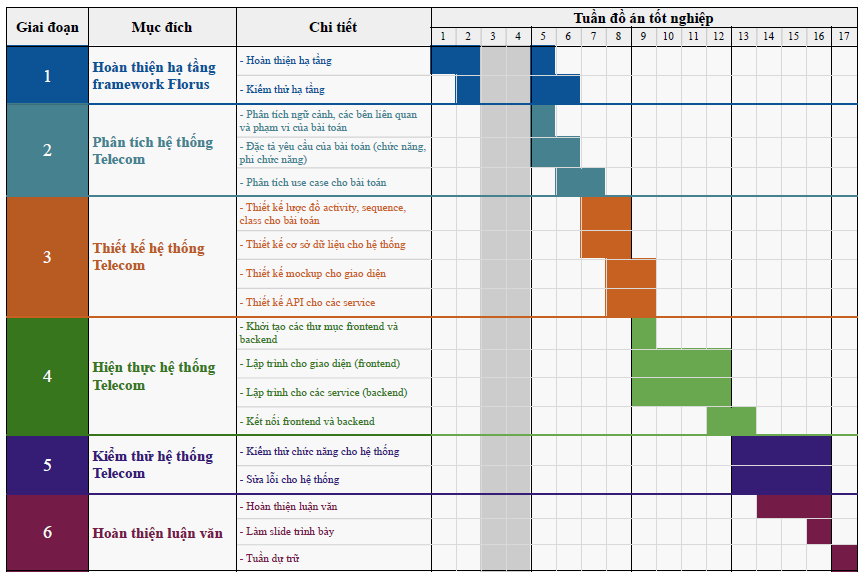
\includegraphics[scale=0.95]{images/gantt.png}
    \caption{Kế hoạch làm việc cho giai đoạn Đồ án tốt nghiệp}
    \label{fig:plan}
\end{sidewaysfigure}